% !TEX root = writing_version.tex

\label{chp:simulation}
During the course of the master thesis an event driven molecular dynamics (EDMD) simulation code has been developed. The EDMD approach is chosen because the actual dynamics of the system is required to search for possible memory effects. This means that simulations only probing the phase space of the system, like Monte Carlo (MC) simulation schemes, are not suited.\\ 
Furthermore the discontinuous potential of the hard spheres is an obstacle not easy to face in regular molecular dynamics (MD) schemes where the Newtonian equations of motion for the particles are numerically integrated. As the EDMD approach even requires these discontinuities it is very well suited for the purpose at hand.\\ 
The key points of the program, possible extensions and a thorough testing are presented in the following, starting with the units of the simulation which are also used throughout this thesis. They are $\sigma$ the sphere diameter as the unit of length, $m$ the mass of a particle as the unit of mass, $k_B T$ as the unit of energy and resulting from these $\delta t = \sqrt{m / (k_B t)} \, \sigma$ as the unit of time.

\section{Algorithm and simulation details}
\label{sec:simulation}
%EDMD and Simulation details
In this section we will highlight the main differences to regular MD simulation schemes which are another main tool to probe the dynamics of molecular systems. Furthermore, we will stick to the hard sphere example when discussing the EDMD simulation but it should be kept in mind that the approach allows to simulate all systems governed purely by potentials made of step functions.\\
 
The decisive difference between EDMD simulations and regular MD schemes is that, instead of evaluating all pair and external forces on each particle and then evolving the whole system accordingly to the next time step, EDMD simulations do not use a predefined time step. Instead, the system is evolved from one event time to the next one which is defined by the next collision of two particles within the simulation box.\\

The employed event prediction algorithm follows the approach proposed by Bannerman et al.2014\cite{Bannerman2014} closely and is discussed in the next section.

\subsection{Event driven molecular dynamics (EDMD)}
\label{sec:EDMD}
For the prediction of events in EDMD simulations an overlap function $f_{ij}(t)$ between particles $i$ and $j$ is defined. It uses the squared quantities because they are easily accessible.\\
\begin{align}
f_{ij}(t) & \coloneqq  | \vec{r}_j(t) - \vec{r}_i(t) |^2 - \sigma^2\\
          & \; \; \, \vrule
  \begin{aligned}[t]
    \quad \text{with} \quad \vec{r}_i(t) &= \vec{r}_i(t_0) + (t-t_0) \; \vec{v}_i(t_0) \, \text{,}\\
    \Delta t \coloneqq & \; t-t_0  \, \text{,} \\ 
    \vec{v}_{ij}(t) &\coloneqq  \vec{v}_j(t) - \vec{v}_i(t) \, \text{,}\\
    \vec{r}_{ij}(t) &\coloneqq  \vec{r}_j(t) - \vec{r}_i(t) \, \text{,}\\
    \Leftrightarrow \quad \vec{r}_{ij}(t) &= \vec{r}_{ij}(t_0) + \Delta t \; \vec{v}_{ij}(t_0)
  \end{aligned}\\
f(t)  & = ( \vec{r}_{ij}(t_0) +  \Delta t \;  \vec{v}_{ij}(t_0))^2 -\sigma^2 \\
\label{eqn:overlap_f}
f(t)  & = |\vec{r}_{ij}(t_0)|^2 + \Delta t ^2 \; |\vec{v}_{ij}(t_0)|^2 - 2 \Delta t \; \vec{r}_{ij}(t_0) \cdot \vec{v}_{ij}(t_0)  -\sigma^2
\end{align}  

The overlap function has the property that it is negative for two particles being closer than their diameter, zero at collision and positive if neither overlapping nor touching. The task to calculate the next collision thus is to calculate the roots of \autoref{eqn:overlap_f}.\\

Solving for $\Delta t$ with $rr \coloneqq |\vec{r}_{ij}(t_0)|^2  $, $vv \coloneqq |\vec{v}_{ij}(t_0)|^2  $ and  $ rv \coloneqq \vec{r}_{ij}(t_0) \cdot \vec{v}_{ij}(t_0) $ has the solution given in \autoref{eqn_delta_t_solution}.
\begin{align}
0 &= rr + vv \; \Delta t ^2  - 2 rv \; \Delta t  -\sigma^2 \nonumber\\
\Leftrightarrow \quad 0 &= \Delta t ^2 - \frac{2rv}{vv} \; \Delta t + \frac{rr - \sigma^2 }{vv} \nonumber\\
\label{eqn_delta_t_solution}
\Leftrightarrow \, \, \Delta t &= - \frac{rv}{vv} \pm \sqrt{\left(\frac{rv}{vv}\right)^2 - \frac{rr - \sigma^2 }{vv}}
\end{align}

A caveat when executing on a floating point machine, however, is present as can be seen when we consider which solution is the relevant one. For a possible collision it is necessary that the two particles move towards each other or mathematically $rv<0$ as the relative velocity is required to be opposite to the relative position.\\

Further the quadratic formula has two solutions, corresponding to the beginning and the ending of the overlap. Due to the entry being prior to the exit, we further conclude that we are interested in the smaller solution which is
\begin{align}
\label{eqn:collision_prediction_pre}
\Delta t &= \frac{ - rv - \sqrt{ (rv)^2  - vv (rr - \sigma^2 )} }{vv} \; \text{.}
\end{align}
Now, for the case where the distance of the spheres is already close to the diameter of the spheres, we find $(rv)^2 \gg (rr-\sigma^2)$ which results in a cancellation of two large numbers leaving a small number. Floating point number operations are inherently badly suited at this point, as they tend to large inaccuracy in this case. However, reformulating \autoref{eqn:collision_prediction_pre} by making use of the third binomial formula, leads to the mathematically identical expression
\begin{align}
\label{eqn:collision_prediction}
\Delta t &= \frac{(rr - \sigma^2 )}{ - rv + \sqrt{ (rv)^2  - vv (rr - \sigma^2 )}} \; \text{.}
\end{align}
Comparably \autoref{eqn:collision_prediction} does not contain a cancellation of the type seen before and hence is better suited for the use in the computer simulation as stated by Goldberg 1991\cite{Goldberg1991}.\\

The event prediction algorithm proposed by Bannerman et al.\cite{Bannerman2014} works by differentiating 4 cases:
\begin{enumerate}
\item If $rv>0$ the particles move away from each other leading to a collision time of $\Delta t = \infty$
\item If $rr<\sigma^2$ an overlap is present resulting in an immediate collision time of $\Delta t = 0$
\item If $(rv)^2  - vv (rr - \sigma^2 ) \leq 0 $ the two particles miss each other, including touching without momentum transfer, resulting in a collision time of $\Delta t = \infty$
\item If none of the before is true the particles collide and $\Delta t$ is calculated by \autoref{eqn:collision_prediction}.
\end{enumerate}

All possible collision times for a particle are then stored in a queue that is sorted by the event times and is called particle event list (PEL). From the PEL the first entry is then passed to the global future event list (FEL).This procedure initially takes place for all particles to set up the system and later on only for those particles involved in the execution of an event.\\

While this is the simplest description in \autoref{sec:implemetation}, the implementation of some widely used measures to reduce redundant calculations and the use of a cell system to reach $\mathcal{O}(N)$ computation time are further discussed.\\

An important detail to take care of is the possibility of scheduled events which have become invalid due to an earlier collision of one of the particles. This is handled by assigning an interaction count to each particle that is stored at precalculation time with the event. When the event is drawn from the FEL and the interaction count of one of the particles has increased in the meantime, the event is said to be invalidated. Depending on which particle had an event in the meantime the invalidation either causes no action or a recalculation of new events.

\subsection{Details concerning the implementation} 
\label{sec:implemetation}
%Add Details of for example FEL, and backupevent handling, double time precision, reset sim
As the simulation code is based on an earlier Monte Carlo code for hard spheres a complete walk through the whole program would be extensive. Hence, we will focus on key points to understand the details of the simulation program. Furthermore, differences to the MC program are mentioned for the readers that are familiar with it.

\subsubsection{The \textit{Event} struct}
\label{sec:event_struct}
We start with the basic \textit{Event} struct which includes 6 entries that are shown in \autoref{tab:event_entries}.
\begin{table}[h!]
\centering
\begin{tabular}{c|c}
\textbf{Datatype} & \textbf{Name of entry}\\ \hline
(double) & time \\
(int) & event\_type \\
(Particle*)  & particle \\
(void*) & partner \\
(int) & particle\_count \\
(int) & partner\_count \\
\end{tabular}
\caption[\textit{Event} struct content]{Content of the \textit{Event} struct.}
\label{tab:event_entries}
\end{table}
The \textit{time} variable holds the time for when the event is scheduled in the future. The \textit{event\_type} variable is either set to 0 or 1 and indicates if the event is a cell transfer or a collision of two particles respectively. To include hard walls or other elements further types of events can be defined.\\
The \textit{particle} variable is a pointer to the particle for which the event has been precalculated, while the \textit{partner} variable is defined as a void pointer. This allows it to either be interpreted as a particle pointer for the collision type event or as an integer pointer to the index in the current cells' neighbors list for transfer events.\\
In the last two rows the interaction counts for particle and partner are listed as well. As the destination cell in a transfer event does not require an interaction count the \textit{partner\_count} variable is only used for collision events.\\

The \textit{event} struct is used for all events throughout the simulation. For read and write operations with the HDF5 file format, the struct \textit{event\_data} is available which uses only indexes instead of pointers.

\subsubsection{The \textit{Particle} class}
\label{sec:particle_class}
The \textit{Particle} class is comparable to the one from the MC code basis. Its MC related attributes have been removed and additional key variables and concepts will be discussed in the following.\\

First, a vector storing events called \textit{backupEvents} has been added to make it possible to store events from the precalculation for the case of the first event being invalidated. The idea of reusing events is discussed in many publications, for example, Bannerman et al. 2011\cite{Bannerman2011} states that the memory cost increases linearly with more backup events while the speedup does not increase much for more than two stored events. It also has been argued that the added complexity can not account for the increase in efficiency Donev et al. 2005\cite{DONEV2005}.\\ 
However, in our own simulations a calculation time reduction of more than 10\% was observed and the cost of complexity and memory was seen as moderate. The difference might be explained by the fact that the systems under consideration in this thesis have a rather large particle density which leads to more invalid collisions.\\

In the context of reusing precalculated results, it should also be mentioned that after a cell transfer the recalculation of events can be reduced to possible partner particles of only the new neighboring cells leading to only 1/3 of the calculation time in this case. But, as the systems under consideration are very dense, transfer events often constitute less than 5\% of all executed events. Thus, the increase in efficiency is assumed to be to costly on the complexity side and not implemented. For sparse systems, however, it might make sense to include an \textit{updatePEL()} routine as transfers are more frequent.\\

Further key differences to the former MC particle type are the variables \textit{total\_interactions} and \textit{particle\_delayed\_time}. The first is the variable for book keeping of interactions. The second is necessary because the particles are not synchronized in time. Nevertheless, the behavior is well defined by the ballistic equation of motion. To actually take the whole configuration to one point of time, the \textit{transferToTime()} function of the particle is provided. This is obviously necessary for measurements including snapshots.\\

This is not a problem because each particle only moves on purely ballistic trajectories until an event occurs and quite on the contrary 

it would mean executing extra operations with extra calculation time and extra rounding errors.\\
To take the whole configuration to one point of time, the \textit{transferToTime()} function of the particle is provided. This is obviously necessary for measurements including snapshots.\\

As mentioned before, the system behaves chaotic even under slightest changes like a rounding error from an extra floating point operation. A result of this is that measuring at different rates during a simulation changes the simulation. It is observed in \autoref{sec:precision} that the system may keep close to the undisturbed trajectory for about 50-100 events/particle. As it is of desire to measure quantities and take snapshots without disturbing the simulation, the program employs copies of the configuration being costly in terms of memory but making simulation resets or higher sampling rates at interesting points possible within a well defined trajectory.\\ 

The measurement without perturbing the system is implemented by making a backup copy of the working configuration just before a measurement is taken. The working trajectory then is disturbed by the measurement and afterwards replaced with its state before the measurement from the backup configuration.\\
A second copy is carried throughout the simulation including the full simulation state to save and reset it at any point during the simulation without writing to the file. This could be useful to do a committer analysis in which a cluster at different stages is sampled multiple times with different perturbations.

\subsubsection{The \textit{Box} class}
\label{sec:box_class}
The box of the simulation remained in principle the same as in the previous MC code. A new element is the \textit{neighbors\_lookup} table which contains the indices to the elements in the cells' array \textit{neighbors} where pointers to the cells that share a surface are stored. It is used to identify which cell a particle has to be transferred to during a cell transfer event.\\

Furthermore the \textit{Update()} routine now takes care of all quantities depending on the length of the box, and the \textit{rescale()} routine is a simple rescaling of the edge lengths with an additional \textit{Update()} call.

\subsubsection{The \textit{Scheduler} class}
\label{sec:scheduler_class}
While the aforementioned elements of the program are also required for the EDMD simulation, the \textit{Scheduler} class certainly contains the most distinct parts of the program. It keeps track of all events to come, predicts new events and orchestrates the execution of the events. The essential functions are discussed in the following subsections while some basic properties are shortly highlighted here.\\

First of all the \textit{Scheduler} holds the future event list (FEL) in which at least one event per particle is stored. As discussed within \autoref{sec:particle_class}, the simulation is capable of saving the complete state of a trajectory, including all precalculated events. For this purpose the \textit{reset\_FEL\_array} is available. Furthermore, the \textit{Scheduler} includes the \textit{global\_time} variable that holds the latest event execution time.\\

We may also note the importance to preallocate all arrays that are used in the event calculations for the efficiency because the collision prediction routine is executed about 30 times per step and particle, and easily accounts to a few billion function calls during a small simulation.

\subsubsection{\quad \textit{Scheduler::predictTransfer()}}
As the name suggests, this function predicts the next cell transfer of a particle due to its movement. It calculates the position of the particle at global time which for a valid state of the simulation always lies within its cell. Denoting for each dimension $i$, the position of a particle within its cell by $r_i$, its velocity by $v_i$, and the cell's length by $l_i$, we can formulate for each dimension the equations
\begin{align}
t_{i1}=-\frac{r_i}{v_i} \quad \text{and} \quad t_{i2}=\frac{l_i-r_i}{v_i} 
\end{align}
which describe the times $t_{i \, 1/2}$ when the particle pierces the cell's left and right boundaries in dimension $i$. A negative time corresponds in this case to a boundary crossing in the past. A time comparable to 0 means that the particle is on the edge of its cell and a positive time means that the boundary crossing lies in the future. By going through the different possible cases for $t_1$ and $t_2$, we find the resulting next crossing time for each case as shown in \autoref{tab:crossing_times}.
\begin{table}[h]
\centering
\begin{tabular}{c|c||c|c}
$t_1$ & $t_2$ & Result & Case \\ \hline
> & > & invalid & - \\ \hline
> & = & $t_{\text{crossing}} = t_1$ & 0 \\ \hline
> & < & $t_{\text{crossing}} = t_1$ & 1 \\ \hline
= & > & $t_{\text{crossing}} = t_2$ & 2\\ \hline
= & = & invalid & - \\ \hline
= & < & $t_{\text{crossing}} = t_1$ & 3 \\ \hline
< & > & $t_{\text{crossing}} = t_2$ & 4 \\ \hline
< & = & $t_{\text{crossing}} = t_2$ & 5\\ \hline
< & < & invalid & - \\ \hline
\end{tabular}
\caption[Cell boundary crossing conditions]{Possible results for left and right crossing time with resulting choice of next crossing time. >, = and < are to be read as for example $t_1 > 0$. The case indicates the case number within the simulation code.}
\label{tab:crossing_times}
\end{table}

By collecting the next crossing times for each dimension and taking the minimum of these times the exit time of the particle from its cell is determined.\\

The return value of the routine is an \textit{Event} where the partner is a pointer to the corresponding entry in the box' \textit{neighbors\_lookup} table. The index is between zero and five corresponding to the six possible neighbor cells sharing a surface with the current cell of the particle. Each valid case represents a distinct neighbor cell and its index within the cell's \textit{neighbors} array is clearly defined by the cell setup routines. The indices within the neighbors array are matched with the defined cases is \autoref{tab:cell_neighbor_index}. 

\begin{table}[h]
\centering
\begin{tabular}{c|c|c|c}
dimension & boundary & case & index \\ \hline
x & front & 0 & 12 \\
 & back & 1 & 13 \\ \hline
y & front & 2 & 10 \\
 & back & 3 & 15 \\ \hline
z & front & 4 & 4 \\
 & back & 5 & 21 \\
\end{tabular}
\caption[Lookup table of cell neighbor indices]{Overview of the cells' \textit{neighbors} indices directly sharing a surface for 3 dimensions. As the indices hardly follow any simple pattern they are explicitly noted at this point. Obviously the cell consists of a front and a back boundary in each dimension. The corresponding case numbers are identical to the ones from \autoref{tab:crossing_times}.}
\label{tab:cell_neighbor_index}
\end{table}
%\FloatBarrier

\subsubsection{\quad \textit{Scheduler::predictCollision()}}
The prediction of collision times has already been discussed in \autoref{sec:EDMD}. The implementation in the program first calculates all necessary scalar products while accounting for the periodic boundary conditions and in a second step returns the collision time depending on the case at hand. While the here presented algorithm is only valid for single sized particles, it can be extended to polydisperse systems as is shown in \autoref{sec:extension_radius}.\\

As this routine is executed throughout the simulation multiple times, it has been tried to optimize its efficiency as far as possible. For example, calculating only necessary results for the next case differentiation has been tried but without significant increase in efficiency and for better readability the prior version has been used instead. In either case, if more efficient calculations are found, it is useful to implement them at this point. 

\subsubsection{\quad \textit{Scheduler::setupFEL()}}
This routine fills the FEL of the simulation. For this purpose it iterates through all particles and calls \textit{setupPEL()} for each of them. The PEL in turn is set up by predicting the next cell transfer as well as the next collisions with all particles within the $3^d$ cells in $d$ dimensions directly surrounding the particle. From all predicted events only such with finite times are then written to the \textit{backupEvents} vector that is the PEL of the particle.\\
For the FEL only the top event of each particle's PEL is then used. Because other events from the PEL might move on to the FEL at later times the top event that was pushed to the FEL has to be erased from the PEL.

\subsubsection{\quad \textit{Scheduler::executeTransfer()}}
The execution of a transfer event is accomplished by the particle's \textit{MoveBetweenCells()} routine. The departure cell is taken as the event particles own cell while the information about the destination cell is contained in the event's \textit{partner} variable. It points to the address within the lookup table of the box where the index of the pointer to the destination cell, in the departure cell's neighbors array, is deposited.

\subsubsection{\quad \textit{Scheduler::executeCollision()}}
The velocity change after a collision between particles i and j of same mass, with corresponding velocities $\vec{v}_{i/j}$ and relative position $\vec{r}_{ij} = \vec{r}_{j} -\vec{r}_{i}$ is given by   
\begin{align}
\label{eqn:collision_result}
\vec{v}_i^{\,'} = \vec{v}_i + \left( \frac{rv}{rr} \right) \vec{r}_{ij} \; \text{,}
\end{align}
where the definitions from \autoref{eqn_delta_t_solution} of the scalar products, $rr$ and $rv$, for the relative positions and velocities are used. An own derivation, also for arbitrary masses, is given in \autoref{eqn:momentum_transfer}, as most textbooks only show the momentum transfer in the center of mass frame.
 
\subsubsection{\quad \textit{Scheduler::executeEvent()}}
The execution of an event works in multiple steps. At first the topmost \textit{Event} is copied from the FEL where it is deleted. Next the validity of the interaction counts of the particle (\textit{cond1}) and its partner (\textit{cond2}) are evaluated. The validation is nothing more than a comparison of the interaction count when the event was scheduled with the present interaction count. The conditions are stored in boolean variables as they are used in the following flow statements. Furthermore, in the case of a transfer event the validation of the partner is not necessary but for better readability performed either way.\\
It follows a distinction between 5 cases which are given by:
\begin{description}
\item[Valid transfer (\textit{event\_type}==0 and \textit{cond1}) ] \hfill \\ The transfer is executed, the global time is evolved to the event time, the particle's PEL is rebuilt and its next event pushed to the FEL.
\item[Valid collision (\textit{event\_type}==1 and \textit{cond1} and \textit{cond2}) ]\hfill \\ The collision is executed, the global time is evolved to the event time, for both participating particles new PEL's are built and each top event is pushed to the FEL.
\item[Invalid transfer (\textit{event\_type}==0 and not \textit{cond1})] \hfill \\ The particle must have had an interaction previously where a new event was scheduled for it, thus no action is taken.
\item[Invalid collision due to particle (\textit{event\_type}==1 and not \textit{cond1})] \hfill \\  The particle must have had an interaction previously where a new event was scheduled for it, thus no action is taken.
\item[Invalid collision due to partner (\textit{event\_type}==1 and not \textit{cond2})] \hfill \\  Only the partner had an interaction previously where a new event was scheduled for it, thus a new event for the particle is required. As the particle had no further interactions, the events in the backup are still valid and the first entry is pushed into the FEL. In case the \textit{backupEvents} array is empty, the PEL is rebuilt and its first entry pushed to the FEL instead.
\end{description}

The order of the cases might be exchanged except for the last two. This is because the last one indirectly assumes \textit{cond1} to be true which is guaranteed by the case before.\\

Furthermore, the routine counts the occurrence of each case, to monitor numbers of collisions, transfers and invalidated cases by type. This is not required by the simulation but can be helpful for understanding the system and simulation.

\subsection{The simulation periphery}
For the simulation to work, some more surrounding is required. This is briefly discussed in the following.
 
\subsubsection{Inout and ch5md}
As suggested by the names, the former comprises the read and write routines of the simulation while the latter one holds routines dealing with the h5md format.

\subsubsection{Setup}
The setup routines are called mainly at the beginning of a simulation to either set up a simulation from a file or to completely start a new simulation. So far only the \textit{FCC\_init()} routine is written which initially places all particles on a fcc lattice and assigns the amplitude of their starting velocities by the equipartition theorem to $|\vec{v}| = \sqrt{3}\frac{\sigma}{\delta t}$. The directions are chosen randomly under the constraint to keep the center of mass at rest.

\subsubsection{Tools}
This is the toolbox of the simulation holding routines to measure quantities like mean squared displacement, radial distribution functions and the cluster finding routine. Functions only used within the simulation like an overlap or minimal distance routine for the compression are included at this point as well.\\

The cluster finding algorithm will be highlighted at this point, as the details of it are necessary to compare the direct data of cluster sizes with the data of other groups.\\ 
It is based on the q6q6-bond-order parameters first described by Steinhardt et al.\cite{Steinhardt1983}.
The local structure around a particle $i$ with $N_b$ neighbors is characterized by the quantity
\begin{equation}
\label{eqn:local_q6}
\bar{q}_{lm}(i) = \frac{1}{N_b} \sum^{N_b (i)}_{j=1} Y_{lm} (\hat{r}_{ij}) \; \text{,}
\end{equation}
where $Y_{lm}(\hat{r}_{ij})$ are the spherical harmonics evaluated in the direction of the relative position of particles i and j in a given coordinate system.

$\bar{q}_{6m}(i)$ suffices to indicate the local fcc structure of hard-sphere crystals. Based on $\bar{q}_{6m}(i)$  a normalized vector $\vec{q}_{6}(i)$ is defined with elements for $m=-6$ to $m=6$ given by
\begin{equation}
q_{6m}(i) = \frac{\bar{q}_{6m}(i)}{ \sqrt{\sum_{m'=-6}^{6} |{\bar{q}_{6m'}(i)})}|  } \; \text{.}
\end{equation}

As a minimum threshold for the scalar product $\vec{q}_6(i) \cdot \vec{q}_6(j)$, we choose 0.6 to identify a pair of particles $i$ and $j$ as ``orientational bonded''. To define a solid particle we set the minimum number of bonded neighbours to be $n_B > 8$, similar to ten Wolde et al.\cite{TenWolde1995} or Schilling et al.\cite{Schilling2011}.

\section{Testing of the simulation code}
\label{sec:probe}
To verify the dynamics of the simulation, we measure the long time diffusion constant and the radial distribution function of the stable hard sphere liquid, as there are measurements and theoretical predictions in the literature to compare with.

\subsection{Diffusive behavior}
\label{sec:diffusion_probe}
The diffusive behavior of particles in a liquid usually can be separated in three distinct regimes. First, the short time diffusion which can be understood as the random movement of the particles within their momentary cage within the fluid. Second, a subdiffusive phase in which the particles are repelled for the first time by their nearest neighbors. And third, the long time diffusion to describe the random propagation of the particles through the fluid over time.\\
   
As the ballistic hard sphere system enters into the long time diffusion almost at once, due to the lack of the suspending fluid, only this is measured. By the definition of a diffusive process, the average mean squared displacement (MSD) of a particle is described by 
\begin{align}
\label{eqn:diffusion}
\langle x^2 \rangle(t) = 2 \, d \, D_L \, t  \, \text{.}
\end{align}
$\langle x^2 \rangle$ is the expectation value of the MSD, $d$ the number of spatial dimensions, $D_L$ the long time diffusion constant and $t$ the system time. With this relation we can use the measurement of $\langle x^2 \rangle (t)$ and take its linear regression to find the diffusion constant $D_L$.

The used testing systems are characterized in \autoref{tab:system_diffusion}. The equilibration phases have been carried out at the final volume fractions up to $\eta = 50\%$ while above this an initial volume fraction of $\eta_i = 45\%$ has been used to obtain a fluid rather than a solid during the equilibration phase. As some measurements are within the metastable regime, it has been checked that no clusters were present in the box during the measurement as they would reduce the averaged diffusion.\\


\begin{table}[h]
\centering
\begin{tabular}{c|c}
Parameter & Value \\ \hline
N & 16384 \\
eq\_steps/particle & 5000 \\
pr\_steps/particle & 20000 \\
$\eta_i$ & 5\% ... 50 \% \\
$\eta_f$ & 5\% ... 54 \% \\
\end{tabular}
\caption[Simulation parameters for diffusion measurement]{Input parameters of diffusion test systems.}
\label{tab:system_diffusion}
\end{table}


The resulting diffusion constants depending on the volume fractions are shown in \autoref{fig:diffusion_const} alongside with values from the literature for the same hard sphere fluid.\\

\begin{figure}[h]
\centering
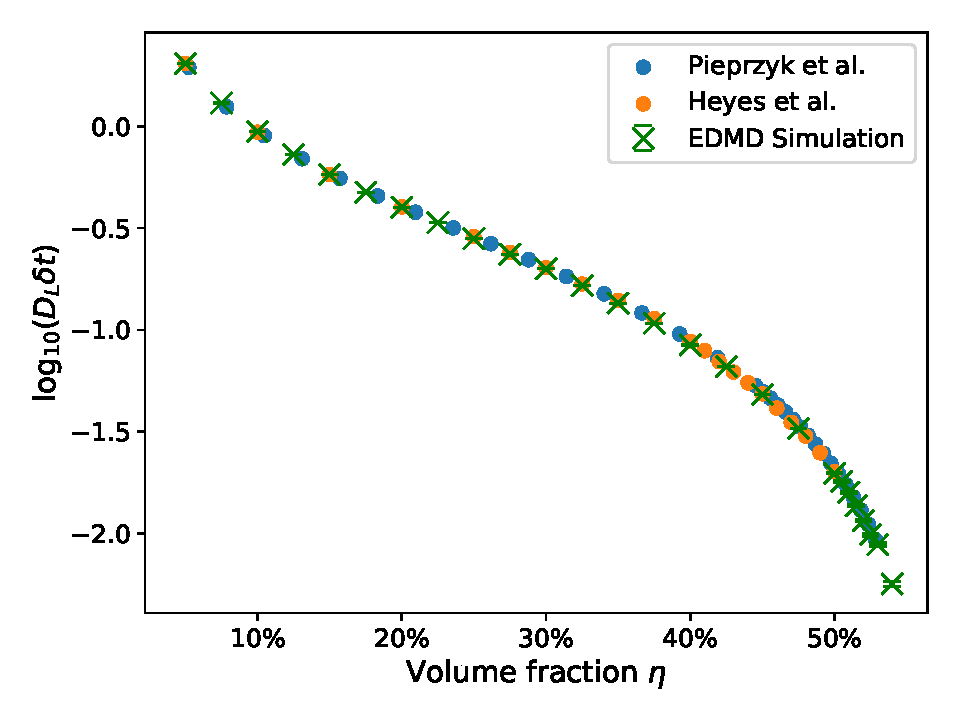
\includegraphics[width=0.6 \linewidth]{diffusion_probe.pdf}
\caption[Long time diffusion constant at varying volume fractions]{Logarithmic plot of long time diffusion constant for the hard sphere liquid as measured in our own simulations as well as measurements from Pieprzyk et al. 2019\cite{Pieprzyk2019} and Heyes et al. 2007\cite{Heyes2007}.}
\label{fig:diffusion_const}
\end{figure}

As it can be seen, the EDMD simulation is capable of reproducing the diffusion constant for the hard sphere liquid. Consequently, we expect the dynamics of it to accurately approximate the purely ballistic hard sphere system.

\subsection{Radial distribution function}
\label{sec:RDF_prob}
A further well known quantity for the hard sphere system is the radial distribution function. It can be described by the theoretical Percus-Yevick approximation which is used for comparison. In \autoref{fig:rdf_overview}, an overview for a range of volume fractions is shown from the same data sets used in \autoref{sec:diffusion_probe}. As expected, no particles come closer than the diameter of a sphere which verifys that no collisions are missed. Furthermore, the liquid shells become more visible for higher volume fractions. At very high volume fractions we also find a new peak at $r < 2 \sigma$ which indicates the local structuring on the path to nucleation.
\begin{figure}[h]
\centering
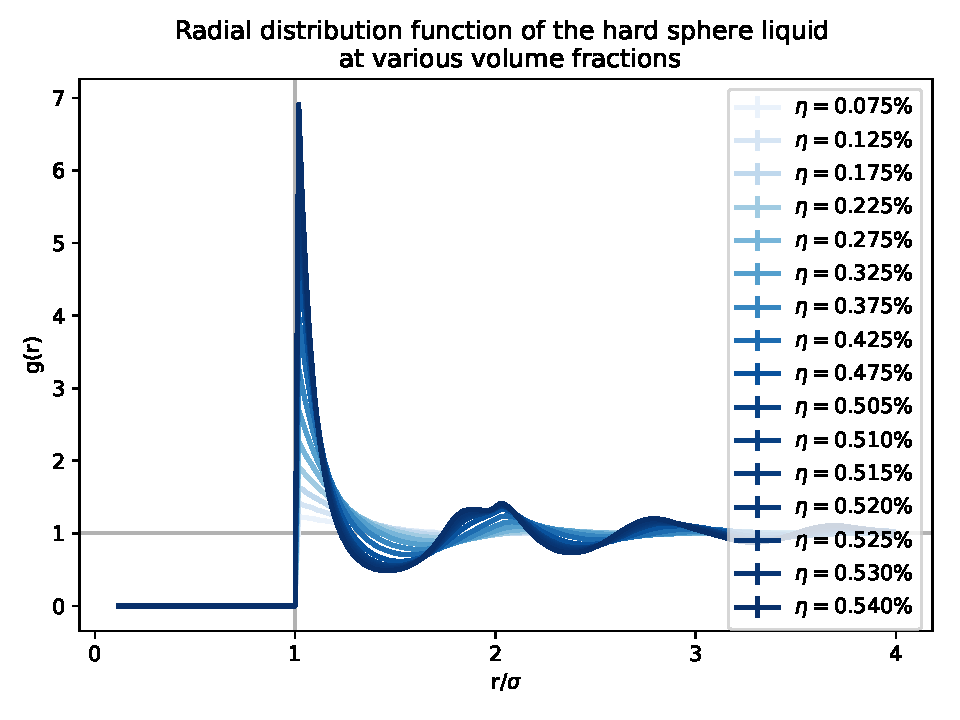
\includegraphics[width=0.7 \linewidth]{RDF.pdf}
\caption[Radial distribution functions at varying volume fractions]{Radial distribution functions for a range of volume fractions, with color lightness corresponding to the volume fraction of the liquid.}
\label{fig:rdf_overview}
\end{figure}
By comparison to the Percus-Yevick approximation, the radial distribution functions for two volume fractions are shown with the corresponding theoretical solution in \autoref{fig:rdf_py}.
\begin{figure}[h]
\centering
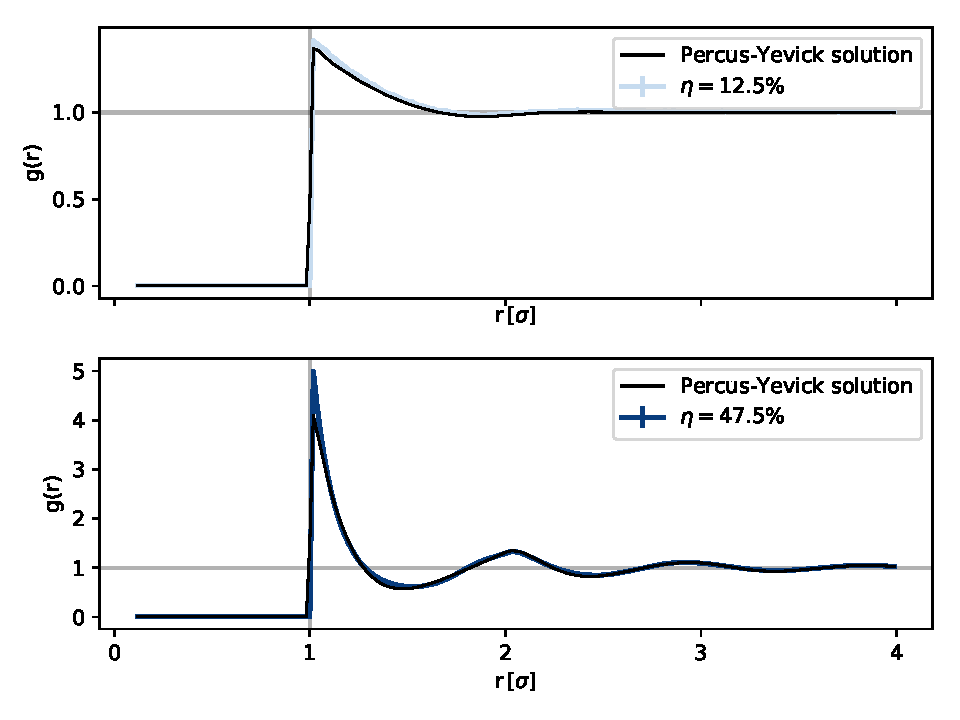
\includegraphics[width=0.7 \linewidth]{RDF_percus_yevick.pdf}
\caption[Radial distribution function with Percus-Yevick approximation]{Radial distribution function of the particles in the hard sphere liquid at a low and at a high volume fraction illustrated along the theoretical Percus-Yevick approximation.}
\label{fig:rdf_py}
\end{figure}
%\begin{figure}
%\begin{center}
%\label{fig:rdf_py}
%\subfloat[Radial distribution functions for a range of volume fractions, with color lightness corresponding to the volume fraction of the liquid.]{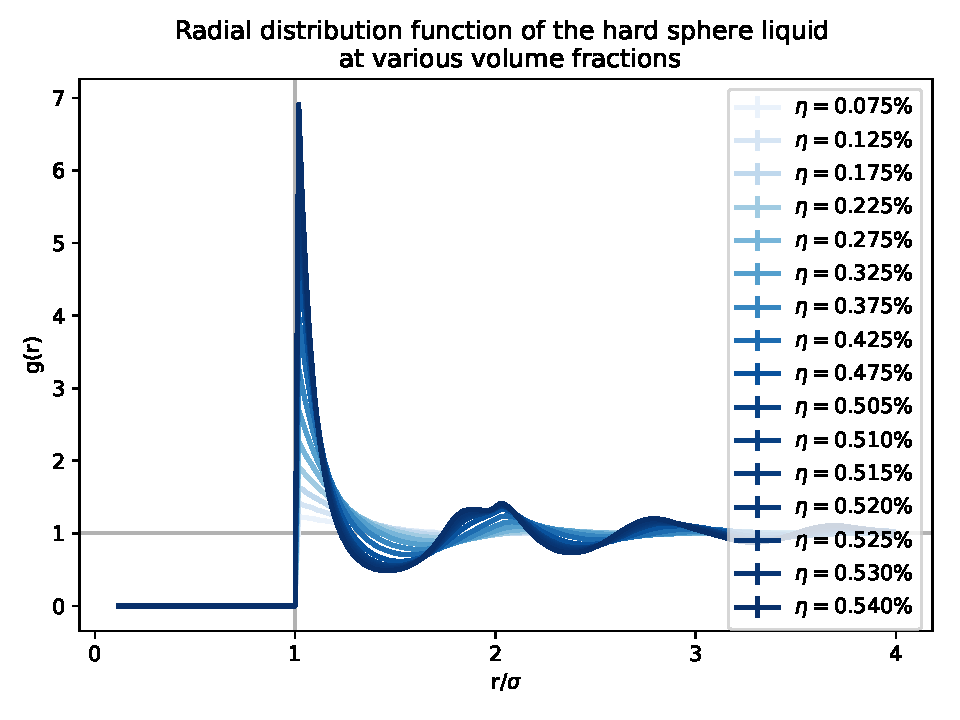
\includegraphics[width=0.45 \linewidth]{RDF.pdf}} \hspace{0.5cm}
%\label{fig:rdf_overview}
%\subfloat[Radial distribution function of the particles in the hard sphere liquid at a low and at a high volume fraction, together with the theoretical Percus-Yevick approximation.]{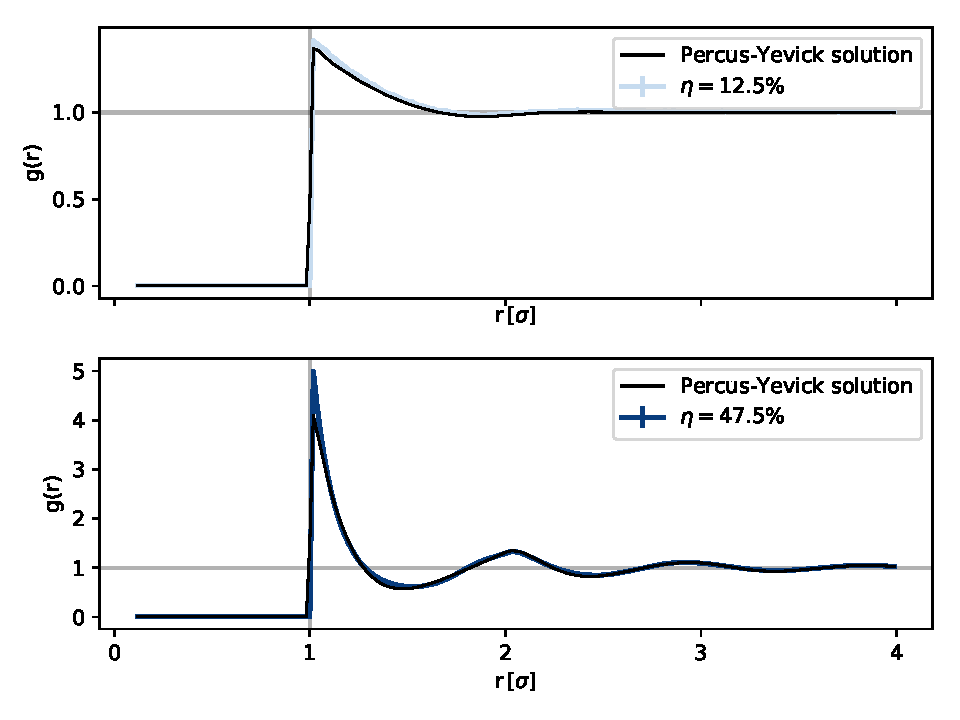
\includegraphics[width=0.45 \linewidth]{RDF_percus_yevick.pdf}}
%\end{center}
%\end{figure}
As highlighted by Hansen and McDonald 2006\cite{Hansen2006}, the theoretical approximation has some flaws as can be seen with $g(r)|_{r=1\sigma}$ being too low for the Percus-Yevick approximation. However, the two radial distribution functions align closely which shows that the developed simulation code is capable of producing accurate data in other contexts as well.
%\FloatBarrier

\section{Estimate of required resources}
\label{sec:resources}
To choose system parameters in a reasonable manner, calculation times and file sizes of the simulation have been characterized. This was necessary as the program was supposed to run on the NEMO high performance computing cluster where hard boundaries are set on calculation times. Therefore, trespasing can cause tremendous loss of data if not correctly caught by the program.
 
\subsection{Calculation time estimate}
\label{sec:calc_times}
The calculation time of the program was tested for a large range of different system sizes up to almost 9 million particles in the fluid state. As can be seen in \autoref{fig:calc_time}, the calculation time increases proportional to the system size for the execution of a step as well as for a measurement in the fluid state. The calculation cost being of $\mathcal{O}(N)$ enables the study of large systems. Furthermore, the execution time of a single event and the measurement time are given by the slopes. As discussed on the example of \autoref{fig:calc_q6q6} the dependence of the measurement routines on the largest cluster size were not seen here as possible clusters remained rather small during these simulation times.\\

\begin{figure}[h!]
\centering
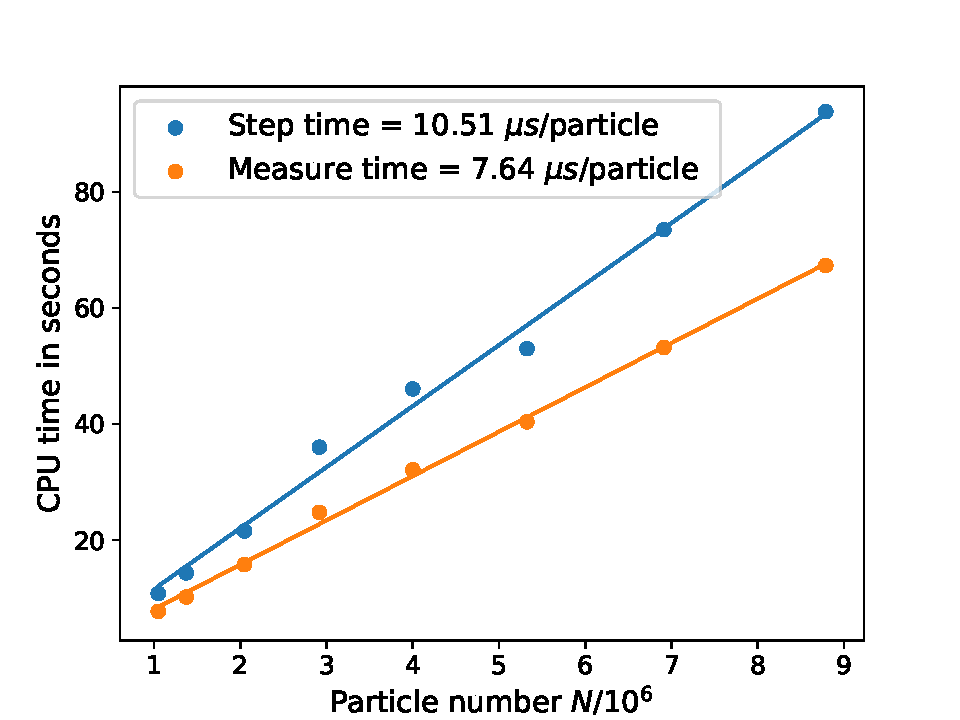
\includegraphics[width=0.6 \linewidth]{Calculation_times_measurement.pdf}
\caption[Calculation time estimate of the simulation]{Overview of CPU time required for calculating a simulation step, consisting of an event for each particle, as well as a measurement of relevant quantities of the system. As assumed for a simulation algorithm with a theoretical $\mathcal{O}(N)$ calculation effort, the data points can be well described by a line. As the CPU time is clearly related to the further workload of the CPU during the calculation it is also expected to find fluctuations if the other workload of the machine is not strictly controlled.}
\label{fig:calc_time}
\end{figure}

The effect of larger clusters was only investigated after problems with the runtime of the programs were traced back to these. The q6q6-order parameter routine was tested for larger clusters in a nucleating simulation with about 1 million particles within the box. As can be seen in \autoref{fig:calc_q6q6}, the calculation cost of the cluster finding routine can be described with a quadratic dependence on the largest cluster. To give an impression of what this means, we can use the calculation costs of a simulation step from \autoref{fig:calc_time} being about $t_{\text{step}} \approx \SI{10}{\mu s \per \text{particle} }$. Therefore, the execution of one step takes about $\SI{10}{s}$ for 1 million particles. If a measurement is performed every 10th step, the calculation cost of the measurements without a large cluster remain below 10\%. But as the largest cluster grows to a few hundred thousand particles in size, the measurements can make up 30\% and more of the calculation cost, or for a fixed number of steps, increase the calculation time by about 50\%. This previously unseen effect lead to actual data loss as the combination of NEMO's policy and EDMD simulation program did not result in a save shutdown of the program after breaching the wall time limit of four days.

\begin{figure}[h!]
\centering
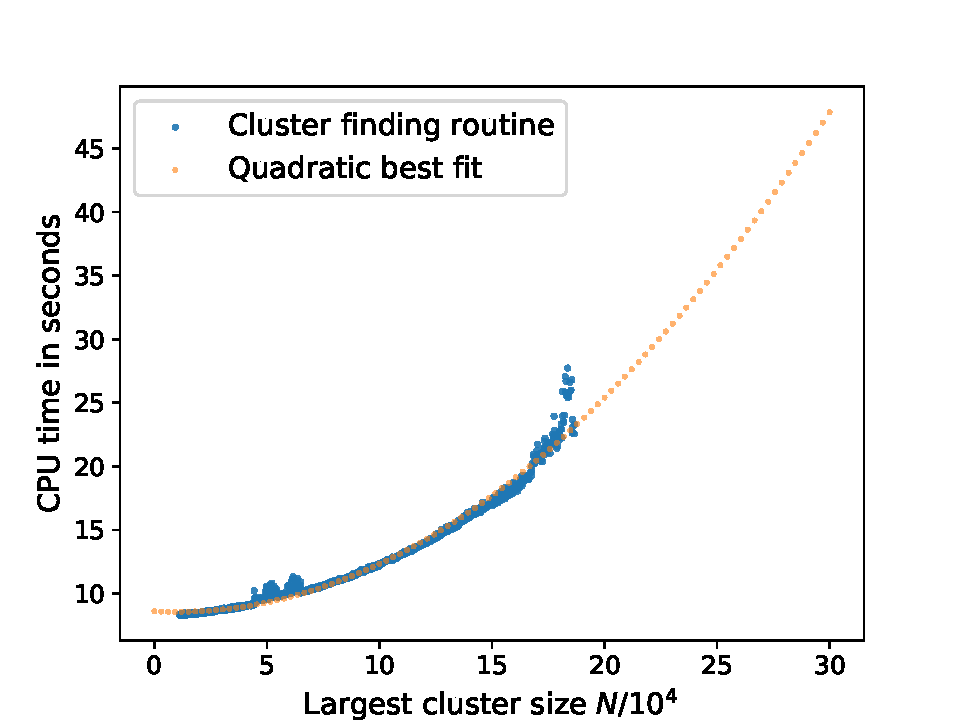
\includegraphics[width=0.6 \linewidth]{q6q6_calculation_time.pdf}
\caption[Quadratic calculation time of q6q6-order parameter cluster finding routine]{Calculation time of the q6q6 order parameter cluster finding routine with an increasing largest cluster size during one nucleation. The quadratic best fit indicates that the calculation effort can be approximated by $\mathcal{O}({N_{\text{lc}}}^2)$, with $N_{\text{lc}}$ being the size of the largest cluster.}
\label{fig:calc_q6q6}
\end{figure}

\subsection{File sizes estimate}
\label{sec:file_size}
A further important constraint for the simulations are the produced amount of data. To get an impression of the file sizes, the required memory for configuration snapshots, reset steps and other measurements were measured prior to the actual simulations. The results of a single snapshot and a single simulation checkpoint are shown in \autoref{fig:file_size}. While the former only contains all positions and velocities the latter contains all positions, velocities, the FEL, all PEL's, delayed times, the cell's first particles and properties of the box. It can be seen that the file size is proportional to the system size as each particle adds a pair of positions, velocities etc. to the saved data.\\
The memory costs of other measurements have been left out of \autoref{fig:file_size}, as these can only amount to substantial file sizes if measurements at each step for long simulations are done. 

\begin{figure}[h!]
\centering
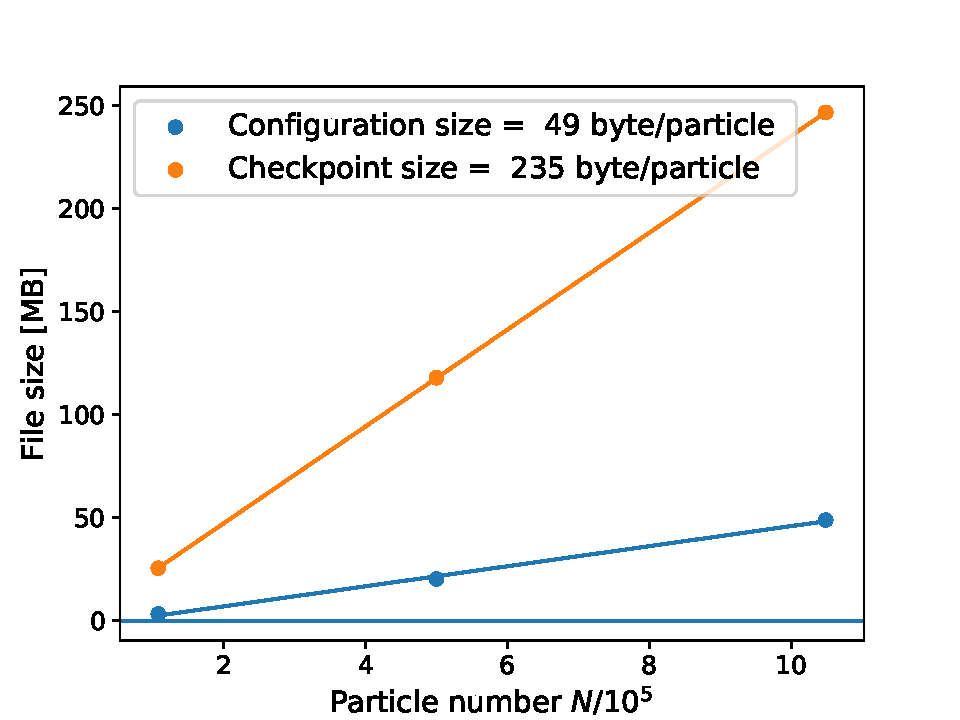
\includegraphics[width=0.6 \linewidth]{File_size.pdf}
\caption[File size estimate of the simulation]{File sizes of a configuration snapshot and a full simulation state at different system sizes with their linear regressions. While for 3 points these are not statistically meaningful, they still remain a useful tool to extract the slope that corresponds to the required memory per particle for a configuration snapshot or a simulation checkpoint.}
\label{fig:file_size}
\end{figure}

\section{Preliminary data for equilibration test}
\label{sec:data}
The motivation to develop the simulation code is based on the interest in nucleation rates of the hard sphere system at varying volume fractions. To observe a nucleation, the volume fraction of hard spheres has to be changed rapidly from lower ones where the system is in the stable fluid phase to higher ones where the stable fluid phase becomes metastable. If this state is evolved in time, nucleations can be observed as stochasticly distributed events. To measure those without artifacts originating from the simulation procedures, some parameters were tested within reasonable ranges prior to the data production.\\
Mainly the number of equilibration steps as well as the initial density before the volume quench are tested because both may impact the local ordering directly after the quench. Thus, we performed some smaller data series to evaluate if and when these effects might come into play.The used test system is characterized by the parameters given in \autoref{tab:system_start_parameter_test}.\\

\begin{table}
\centering
\begin{tabular}{c|c}
Parameter & Value \\ \hline
N & 16384 \\
eq\_steps/particle & 100 ... 20000 \\
$\eta_i$ & 5\% ... 49 \% \\
$\eta_f$ & 54 \% \\
\end{tabular}
\caption[Simulation parameters for testing equilibration step number and initial density]{Input parameters of test systems probing the dependence on equilibration steps and initial density.}
\label{tab:system_start_parameter_test}
\end{table}

The general behavior of the fluid is analyzed by inspecting the cluster size distribution over time. Its average over all trajectories is shown in \autoref{fig:pnt_mean} together with the same data smoothed by a Gaussian filter matrix. The smoothing is employed afterwards, as otherwise only fluctuations are visible at low count rates.\\

\begin{figure}[h!]
\centering
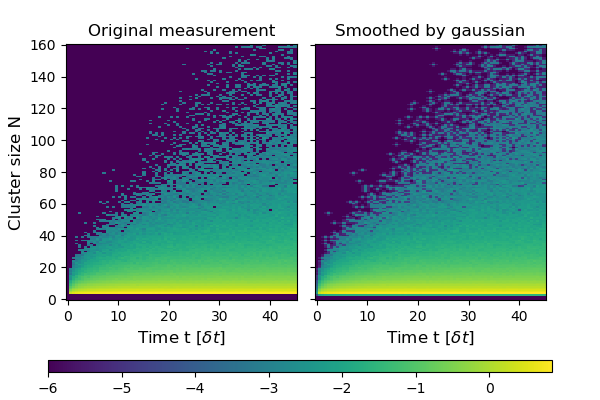
\includegraphics[width=0.6 \linewidth]{mean_pnt.png}
\caption[Gaussian filter applied to cluster size distribution]{Heat map of the mean cluster distribution over time. The diagram encompasses 800 trajectories of 16384 particles each. The coloring indicates the decadic logarithm of the average cluster occurrence in a box which corresponds to a free energy in the stationary case.}
\label{fig:pnt_mean}
\end{figure}

From \autoref{fig:pnt_mean} we can see the reaction of the fluid after the quench into the metastable state. As there are rarely any clusters present in the stable liquid and the spatial configuration of the particles requires some time to rearrange into the local ordering, no clusters are found directly after the quench. In the later evolution we then see how clusters form, and soon after begin to nucleate leaving the y-axis range of the diagram.\\

To identify differences between the ensembles with varying start parameters, the quantity defined in \autoref{eqn:pnt_delta} is used. To circumvent complications due to zero values, they are fixed to values below the regular signal. Three samples of this comparison are shown in \autoref{fig:pnt_eq_step_comparison} and \autoref{fig:pnt_rho_comparison} for different lengths of equilibration phase and different initial densities. The coloring indicates the value of $\Delta_{p(N,t)}$ defined in \autoref{eqn:pnt_delta}. As mentioned before, the quantities $p_i(N,t)$ and $\langle p(N,t) \rangle$ are smoothed by a Gaussian filter because the number of included samples is with 100 trajectories per series not sufficient to produce smooth distributions at the given sampling rate. Thus, without smoothing mostly fluctuations are visible.
\begin{align}
\label{eqn:pnt_delta}
\Delta_{p(N,t)} = \text{log} \left( \left| \frac{p_i(N,t)}{\langle p(N,t) \rangle} -1 \right| \right)
\end{align}
\begin{figure}[h!]
\centering
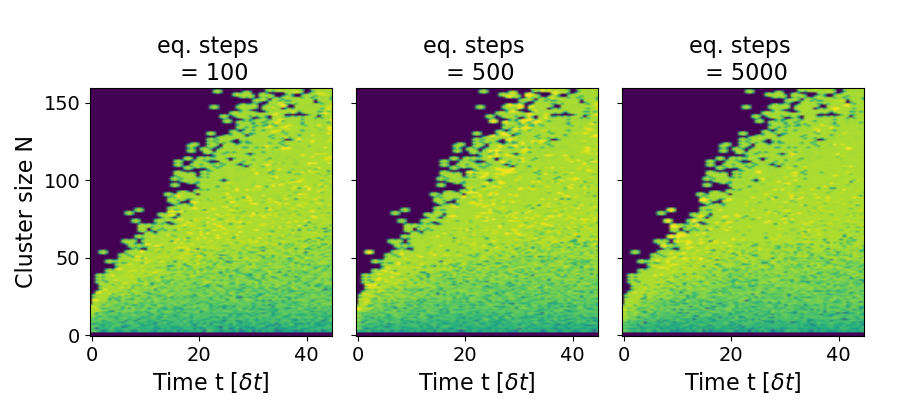
\includegraphics[width=0.7 \linewidth]{pnt_comparison_eq_steps.png}
\caption[Heat maps of differences under variation of equilibration step number]{Heat map of differences between the cluster distributions within simulations carried out with varying lengths of the equilibration phase. The quantity used for coloring is defined in \autoref{eqn:pnt_delta}. Yellow indicates a large difference, whereas blue indicates a small difference. Providing a legend of the coloring is omitted as $\Delta_{p(N,t)}$ has no further use than to indicate differences and actual values do not add any use.}
\label{fig:pnt_eq_step_comparison}
\end{figure}

\begin{figure}[h!]
\centering
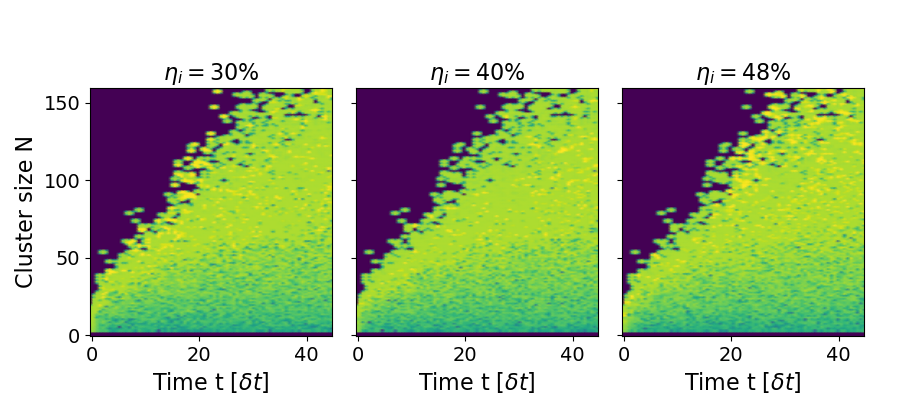
\includegraphics[width=0.7 \linewidth]{pnt_comparison_rho.png}
\caption[Heat maps of differences under variation of initial density]{Heat map of differences between the cluster distributions within simulations carried out with varying the volume fraction of the liquid during the equilibration phase. The quantity used for coloring is defined in \autoref{eqn:pnt_delta}. Yellow indicates a large difference while blue indicates a small difference. Providing a legend of the coloring is omitted as $\Delta_{p(N,t)}$ has no further use as to indicate differences and actual values do not add any use.}
\label{fig:pnt_rho_comparison}
\end{figure}

On first sight, none of them differ in their general behavior. The blue region in the top left corner indicates no difference between the simulations directly after the quench because no clusters were present in the stable liquid and also no clusters have formed yet. The features visible on the edge between the zero region and the nonzero region on the other side are the same, because they are features of the mean distribution shining through. Actual differences that are not due to fluctuations would only be visible within the green and yellow non-zero region, but no such difference is observed.\\

While it seems like the set for an initial volume fraction of $\eta=0.4$ and $\text{eq. steps} = 5000$ includes a little less irregular fluctuations, strong differences remain absent. Especially interesting is the ensemble with $\text{eq. steps} = 100$ because here the length of the equilibration phase is similar to the time the initial perfect crystal configuration takes to melt. For this reason, one could expect that a significant part of these configurations might directly crystallize again but instead we do not find any significant impact.\\

A more quantitative analysis is given by calculating the mean nucleation rates for each set of trajectories. The maximum likelihood estimator that is used for this purpose as well as its uncertainty is discussed in \autoref{sec:ml_estimator}. The results for the different data sets are depicted in \autoref{fig:comparison_nucleation_rates}.
\begin{figure}[h!]
\centering
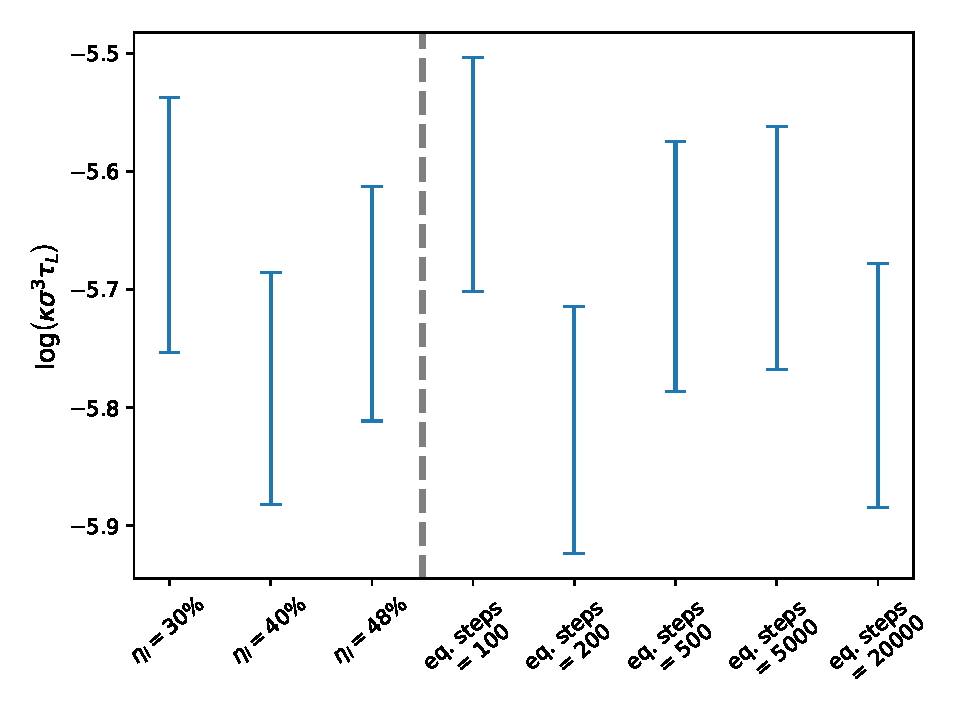
\includegraphics[width=0.45 \linewidth]{nucleation_rate_pre_comparison.pdf}
\caption[Nucleation rates of equilibration test measurements]{Comparison of nucleation rates under CNT assumptions for different initial densities during equilibration with eq. steps fixed at 5000, as well as varying eq. steps with $\eta_i$ fixed at 45\%. }
\label{fig:comparison_nucleation_rates}
\end{figure}

As we can see, no significant difference can be observed between the nucleation rates even for the extreme short equilibration phase of 100 events per particle. For this bold setting the rate is a little higher but still in accordance with the other measurements within its statistical uncertainty.\\

Overall, we can conclude in this chapter that as long as parameters are set within broadly but reasonable boundaries no systematic influence is expected. 

\section{Extensions for future studies}
\label{sec:simulation_ext}
The program at this state is capable of simulating large systems including compression and relaxation. While it has been used to study the nucleation of the monodisperse hard sphere fluid in this thesis, additional features have been developed to suit the code for further studies. Polydispersity in the sense of radius and mass distributions have been implemented and roughly tested, as well as individual cluster tracking, to enable a detailed study of spatial information regarding the clusters. The state of these two features and their use are described in the following two sections.

\subsection{Polydispersity for varying radius and mass}
\label{sec:extension_radius}
Polydispersity has been included in the simulation to make it more comparable to actual experiments in which monodisperse spheres are practically not achieved. Also, the phase diagram becomes richer as the complexity of the system increases as is shown for example by Pusey et al. 2009\cite{Pusey2009}.\\ 
Within the implementation, the prediction of collisions has to be adjusted. When looking at the derivation of \autoref{eqn:collision_prediction} it is found that $\sigma$ being the former diameter of a sphere in the monodisperse case only has to be changed to $\sigma=R_i+R_j$. In \autoref{eqn:collision_prediction2} and \autoref{eqn:var_mass} the same definitions of scalar products are used as before in \autoref{sec:EDMD} where the monodisperse case is discussed.

\begin{align}
\label{eqn:collision_prediction2}
\Delta t &= \frac{\left(rr - (R_i+R_j)^2 \right)}{ - rv + \sqrt{ (rv)^2  - vv \left(rr - (R_i+R_j)^2 \right)}}
\end{align} 

Then, in a physical model with particles that are constituted by some matter with constant density the change of radius is also accompanied by a change of the mass. This has to be taken into account when assigning the velocities after a collision as shown in \autoref{eqn:var_mass}.

\begin{align}
\label{eqn:var_mass}
\vec{v}_i{\,'} = \vec{v}_i + \frac{2 m_j \; (rv)}{(m_i + m_j) (R_i+R_j)^2} \cdot \vec{r}_ij \nonumber \\
\vec{v}_j{\,'} = \vec{v}_j + \frac{2 m_i \; (rv)}{(m_i + m_j) (R_i+R_j)^2} \cdot \vec{r}_ij
\end{align}

A small caveat is given by the fact that the system with different masses requires a new routine to fix its center of mass frame. If this is not considered, unnecessary transition events have to be calculated.

\subsection{Single cluster tracking algorithm}
\label{sec:tracking}
Following trajectories of single metastable clusters within the fluid can be used to measure their mean lifetimes. Also, the nucleation time can be observed with higher precision as the precursor can be tracked back to only a few particles.\\ 
To track individual clusters, they have to be identified in each measurement step because they form out of the liquid and are not numbered and easily distinguishable as the particles are. For this purpose we can either employ the clusters' participating particles or their center of mass positions. The latter one is used as it is easier to compare and to access in our case because a routine to calculate the center of mass of a cluster already is implemented. Furthermore, less data has to be written and compared. An algorithm based on maximum movement from one time step to the other is tested and yields reasonable results as can be seen in \autoref{fig:cluster_tracking_example}.\\

\begin{figure}[h]
\centering
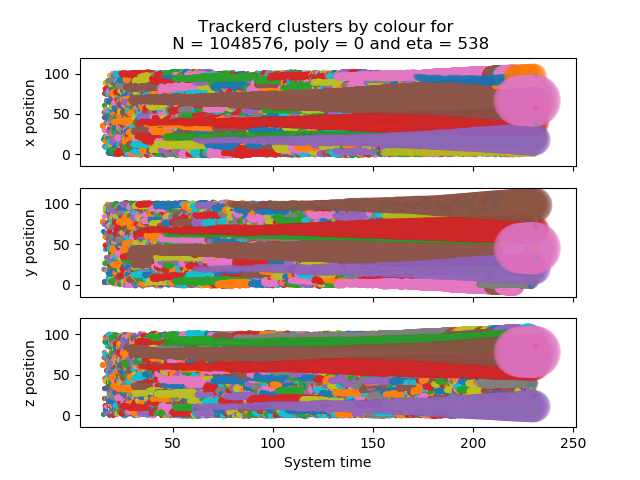
\includegraphics[width=0.6 \linewidth]{cluster_tracking_example.png}
\caption[Individual cluster tracking example]{Example results of the cluster tracking algorithm in a monodisperse simulation. The three plots are the projections of the box onto the three spatial dimensions over time. Each cluster is given a color to identify it. With it we can see for example that two clusters mingling in one projection are actually some distance apart from each other in an other dimension.\\
In this example only small metastable clusters that dissolve after some time are present but also nucleation events can be visualized in this kind of plot. These are easily identified as the width of the line is proportional to the diameter of a sphere with a volume corresponding to the clusters volume under the assumption of it being spherically symmetric.}
\label{fig:cluster_tracking_example}
\end{figure}
Information about the lifetime and size of the fluctuations derived from the analyzed example trajectory shown in \autoref{fig:cluster_tracking_example} are depicted in \autoref{fig:lifetime}.\\
\begin{figure}[h]
\centering
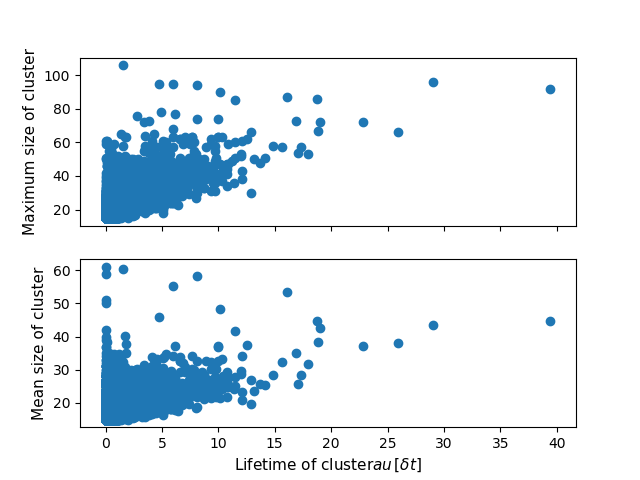
\includegraphics[width=0.6 \linewidth]{cluster_tracking_lifetime.png}
\caption[Example of correlation between an unstable cluster's size and lifetime]{Example of lifetime depending on  maximum (top) or mean (bottom) size of the metastable cluster. The size is defined by the number of particles in the cluster.}
\label{fig:lifetime}
\end{figure}
First we note that both the maximum size and the mean size can be used to measure the scale of the fluctuations as the results mostly vary by the scaling. Further, we can extract from the diagram that at a volume fraction of $\eta = 53.4\%$ there are a lot of small to medium and few large sized clusters. The small ones show short lifetimes up to about $10 \delta t$, while some large ones show lifetimes of more than $15 \delta t$. The large fluctuations with short lifetimes might be caused by merging and splitting of clusters because the simple algorithm does not test for such. The overall impression is that the fluctuation distribution is compact with a small but very far reaching tail towards the large lifetimes as well as towards the large cluster sizes.
\FloatBarrier



